\chapter{Evaluación y experimentación}

En este capítulo se va a explicar cómo de bien funciona el software desarrollado a través de pruebas de carga. Con estas pruebas, se podrá mostrar como rinde
el sistema y cuáles son sus tiempos de respuesta, entre otras medidas más.

\section{Locust}

\textbf{Locust} es una herramienta de código abierto que permite realizar tests sobre una aplicación. El comportamiento es definido a través de un script en Python
y permite evaluar cómo rinde el sistema ante muchas peticiones de usuarios simultáneos.

Para poder usarlo, se ha tenido que instalar la dependencia de locust en un entorno virutal en Python y, además, se han creado dos archivos. Estos archivos son los
siguientes:

\begin{itemize}
    \item \textbf{Locust\_login.py:} este archivo se encarga de hacer un inicio de sesión ejecutando el endpoint de \textit{login} del backend. El contenido del 
    archivo es el siguiente:
    
    \begin{verbatim}
        import os
        from locust import HttpUser, between, task

        class LoginUser(HttpUser):
            wait_time = between(1, 2)

            def on_start(self):
                self.email = os.getenv(
                    "LOCUST_EMAIL", 
                    "canomelero1@gmail.com"
                )
                self.password = os.getenv(
                    "LOCUST_PASSWORD", 
                    "Prueba123"
                )

            @task
            def login(self):
                with self.client.post(
                    "/api/auth/login",
                    json={
                        "email": self.email, 
                        "password": self.password
                    },
                    name="/api/auth/login",
                    catch_response=True,
                ) as response:
                    if response.status_code != 201:
                        response.failure(
                            f"login fallo: {response.status_code}
                                {response.text}"
                        )
                        return

                    data = response.json()
                    
                    if not data.get("accessToken"):
                        response.failure("login sin accessToken")
    \end{verbatim}

    La explicación del código es la siguiente:

    \begin{enumerate}
        \item Se importan las librerías con las que se van a trabajar. Destacando las de locust, encontramos: 
        
        \begin{itemize}
            \item \textbf{HttpUser:} es una clase que representa un usuario simulado haciendo peticiones HTTP. Al crear una clase que 
            hereda de ella, se obtiene el cliente HTTP con el que realizar las peticiones.

            \item \textbf{Between:} es una función que permite definir el tiempo de espera entre las tareas de un usuario, es decir, después de que el 
            usuario realice la tarea de login, esperará de un tiempo aleatorio entre 1 y 2 segundos.

            \item \textbf{Task:} es un decorador que indica al usuario qué funciones va a ejecutar repetidamente.
        \end{itemize}

        \item Se crea la clase que hereda de HttpUser, es establece el tiempo de espera entre cada tarea y se definen los atributos \textit{email} y \textit{password},
        que serán inicializados con los valores que haya en un archivo \textit{.env}, o en caso de no haberlo, con el valor establecido por defecto.

        \item Se crea la tarea de \textbf{login}. Esta tarea se va a encargar de hacer una petición al endpoint de login a través del cliente HTTP creado. En caso de que
        la respuesta obtenida no tenga un código 200 o no tenga el campo de \textit{accessToken} del JSON, dará un error.
    \end{enumerate}

    \item \textbf{Locust\_plots.py:} este archivo va a realizar un test sobre un endpoint del backend para obtener todas las parcelas de un usuario concreto. Se va a definir
    una sola tarea que es la petición al endpoint; sin embargo, para realizar la petición, es necesario iniciar sesión previamente (requiere autenticación) y extraer el ID del
    usuario logueado, por lo que se están realizando dos peticiones antes de obtener las parcelas.

    Con este test se puede comprobar el funcionamiento del sistema cuando se está realizando un trabajo más complejo (mayor número de consultas) y se está devolviendo una mayor
    cantidad de información a un mayor número de usuarios.
\end{itemize}

\section{Ejecución y análisis de resultados}

Para ejecutar los archivos, se escribe la sentencia \textbf{locust -f nombre\_archivo.py} desde la terminal. A continuación, se abre un navegador web y se escribe la
URL \textbf{http://localhost:8089} (o la IP junto con el puerto que es indicado desde la terminal).

Si se han seguido estos pasos, aparecerá en la pantalla lo siguiente:

\begin{figure}[H]
    \centering
    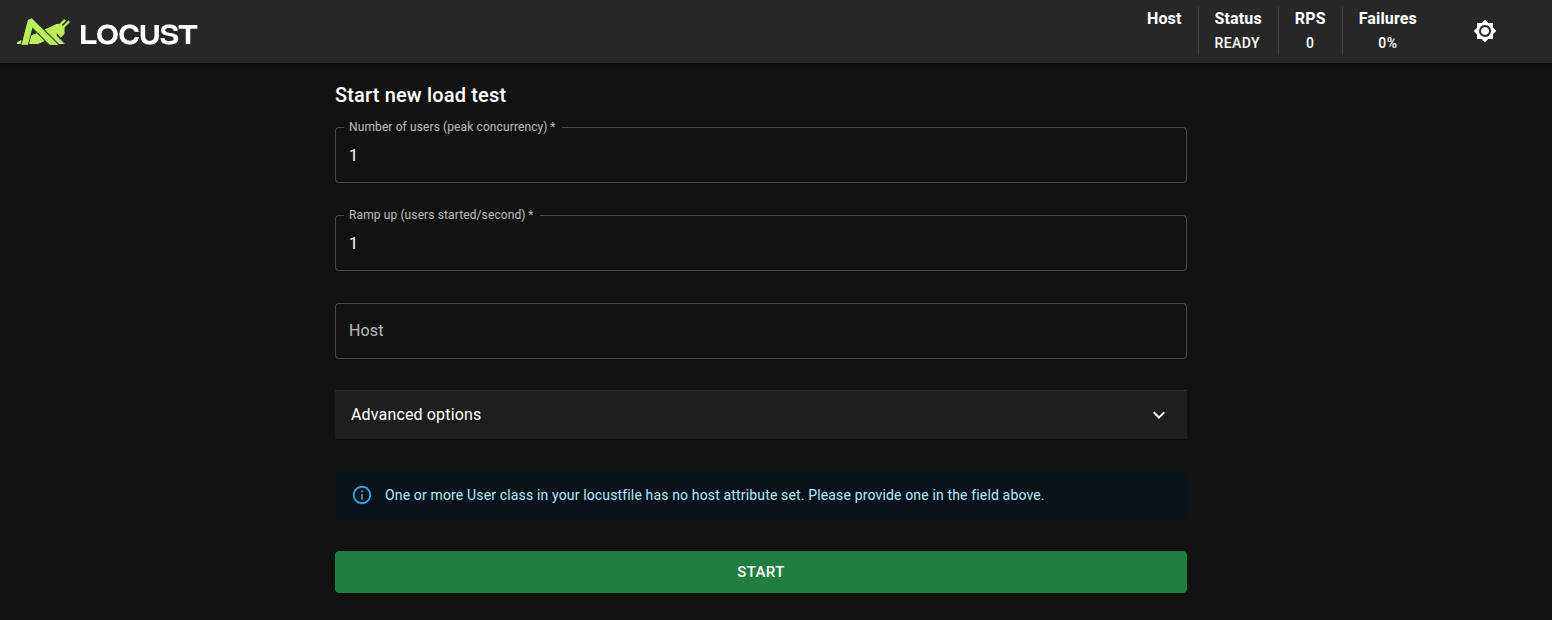
\includegraphics[width=0.9\textwidth]{figures/locust_home.png}
    \caption{Inicio de Locust}
    \label{fig:locust_home}
\end{figure}

En esta interfaz se pueden ajustar los siguientes parámetros:

\begin{itemize}
    \item \textbf{Número de usuarios:} establece cuántos usuarios concurrentes van a realizar la ejecución de la tarea establecida en el script.
    \item \textbf{Ramp up:} establece el tiempo en segundos en el que se van a ir añadiendo los usuarios de manera progresiva.
    \item \textbf{Host:} indica a sobre qué dominio se van a realizar las peticiones.
\end{itemize}

Se empezó ejecuntado el script de login para 100 usuarios y un \textit{ramp up} de 10, de manera que cada 10 segundos, se iban a ir añadiendo usuarios de forma progresiva
hasta llegar a un límite de 100.

Los resultados obtenidos fueron los siguientes:

\begin{figure}[H]
    \centering
    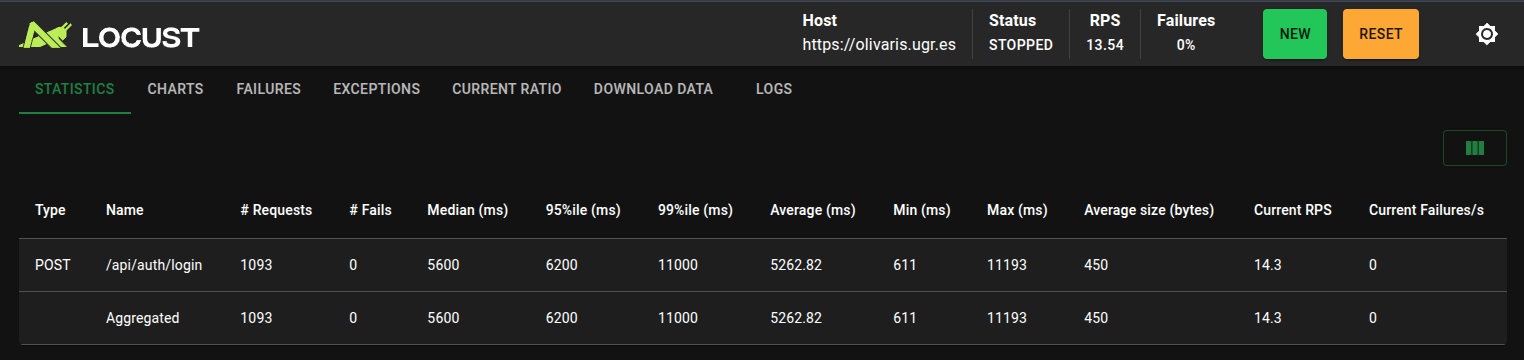
\includegraphics[width=0.9\textwidth]{figures/statistics_100_login_csirc.png}
    \caption{Estadísticas para 100 usuarios en el login desde el CSIRC}
    \label{fig:statistics_100_login_csirc}
\end{figure}

Con estos datos obtenidos se interpreta lo siguiente:

\begin{itemize}
    \item \textbf{Request y failures:} el sistema ha procesado 1093 peticiones de login y no ha habido ningún error. Esto quiere decir que todas las respuestas tenían un código 201
    y que todas ellas contenían el \textit{accessToken} entre sus campos.

    \item \textbf{Median:} indica que el tiempo de respuesta de media es de 5.2 segundos, siendo un tiempo muy alto para una operación de inicio de sesión.
    
    \item \textbf{95\%ile:} esto indica que el 95\% de las peticiones tardaron menos de 6.2 segundos en resolverse. Este dato indica que en general es estable el sistema debido a que
    no hay mucha variabilidad aunque el tiempo sea alto.

    \item \textbf{99\%ile:} indica que el 99\% de las peticiones tardaron menos de 11 segundos. 
    
    \item \textbf{Min y Max:} estos datos indican el tiempo mínimo o más rápido de una petición (611ms) y el tiempo más alto o más lento en procesar una petición (11s).
    
    \item \textbf{RPS:} indica el número de peticiones que el backend está procesando o ``soportando'' por segundo, es decir, procesa 14 peticiones de login cada segundo.
\end{itemize}

Como se puede observar, tiempos de respuesta de 5 segundos aproximadamente para una operación de login con 100 usuarios es demasiado alto. Estos resultados se obtuvieron ejecutando
el sistema desde un servidor proporcionado por el CSIRC, por lo que se pasó a probarlo en local y descartar posibles errores en la arquitectura del sistema, en \textit{querys} a la 
base de datos o en el código.

Ejecutando el mismo script con los mismo datos de usuarios y ramp up pero en localhost, se obtuvieron los siguientes resultados:

\begin{figure}[H]
    \centering
    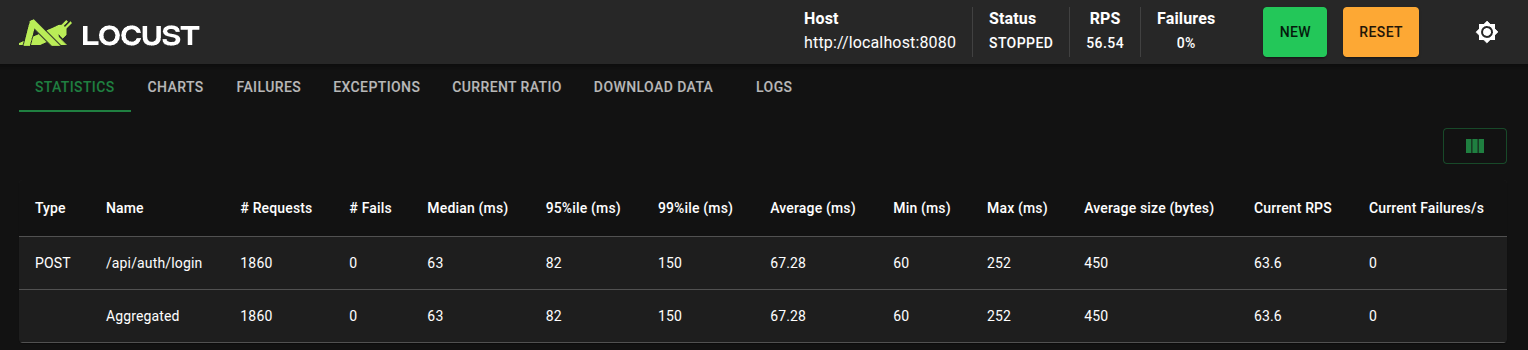
\includegraphics[width=0.9\textwidth]{figures/statis_100_login_local.png}
    \caption{Estadísticas para 100 usuarios en el login desde localhost}
    \label{fig:statis_100_login_local}
\end{figure}

En esta imagen se pueden apreciar resultados más lógicos para un login. Es cierto que es sobre mi PC en local, por lo que no hay una gran latencia pero los resultados se acercan más a
la realidad.

Una vez comprobado que los tiempos son más razonables en local, se hizo la misma prueba pero desplegando el sistema en otro servidor \textit{on-premise} proporcionado por el Juan Luis Laredo,
tutor del presente Trabajo de Fin de Grado. Al ejecutar en este servidor el script con los mismos parámetros se obtuvieron los siguientes resultados:

\begin{figure}[H]
    \centering
    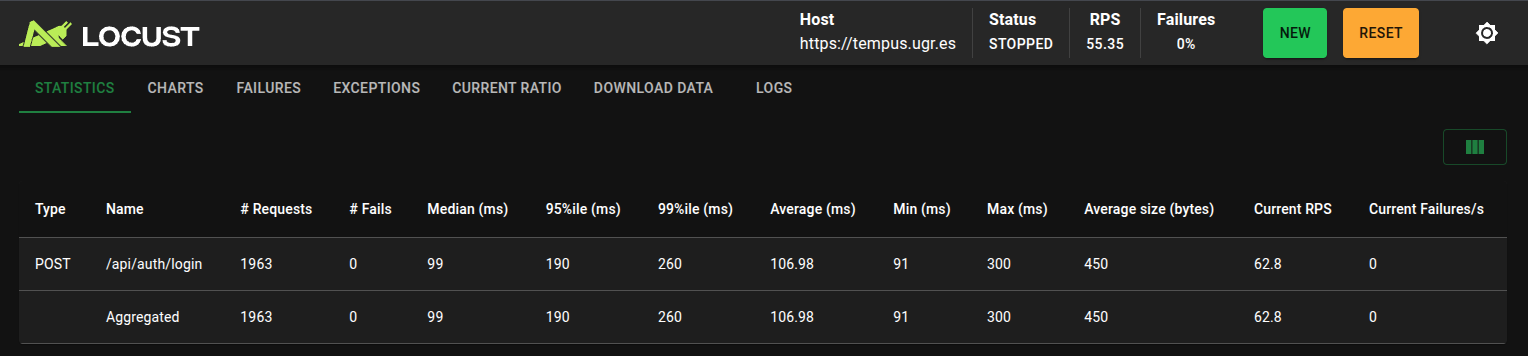
\includegraphics[width=0.9\textwidth]{figures/statis_100_login_tempus.png}
    \caption{Estadísticas para 100 usuarios en el login desde on premise}
    \label{fig:statis_100_login_tempus}
\end{figure}

En este servidor se puede observar como los datos obtenidos son también más razonables para un login con 100 usuarios, ya que se tienen tiempos de respuesta que no llegan a 1 segundo.

Con estas pruebas realizadas tanto en local como con un servidor \textit{on premise}, se descartó la hipótesis de fallos en arquitectura o en código y se dedujo que el servidor del CSIRC
tiene unas prestaciones más reducidas, causando de esta manera tiempos de respuesta bastante más altos que en otras infraestructuras.

\subsection{Comparación de tiempos en el servidor on premise}

A continuación, se va a proceder a ejecutar el script del login en el servidor \textit{on premise} bajo dos condiciones distintas: en una se tendrá 1000 usuarios con un ramp up de 10s, y en otra
se tendrán también 1000 usuarios pero con un ramp up de 100s. Con estos datos se busca ``estresar'' el servidor para ver hasta qué punto puede atender peticiones bajo tiempos de respuesta razonables.

Los resultados con 1000 usuarios y ramp up de 10s son los siguientes:

\begin{figure}[H]
    \centering
    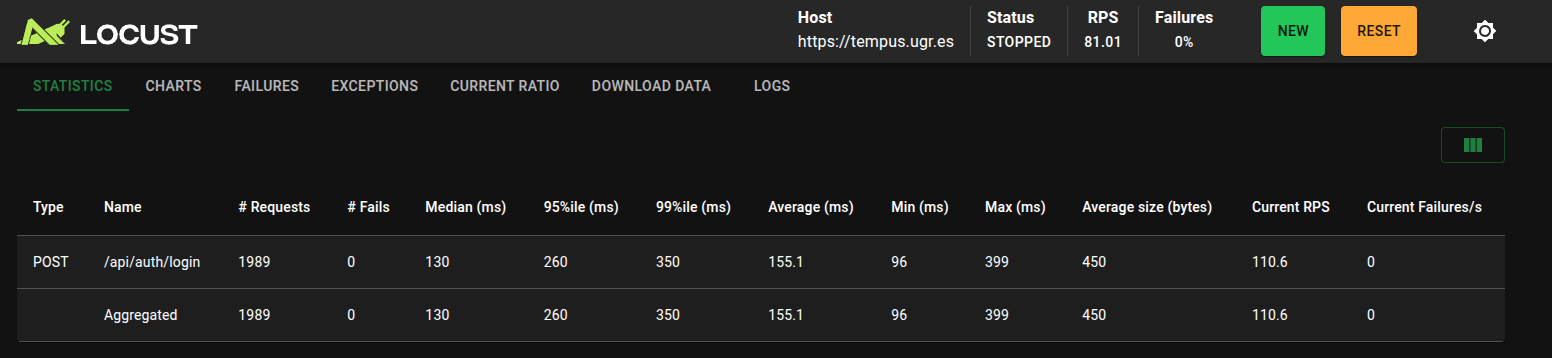
\includegraphics[width=0.9\textwidth]{figures/statis_1000_10_login_tempus.png}
    \caption{Estadísticas para 1000 usuarios en el login desde on premise}
    \label{fig:statis_1000_10_login_tempus}
\end{figure}


Sin embargo, los resultados con 1000 usuarios y ramp up de 100s son los siguientes:

\begin{figure}[H]
    \centering
    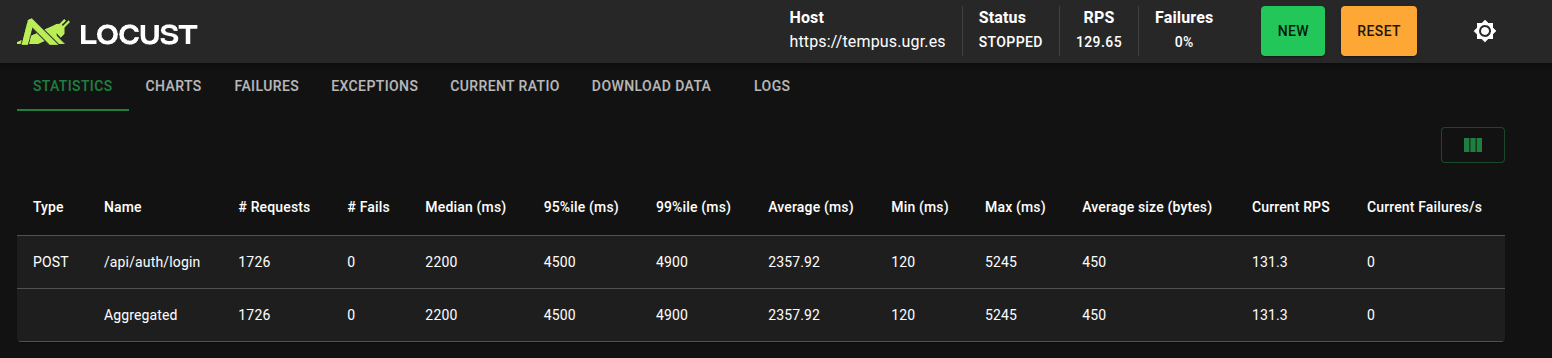
\includegraphics[width=0.9\textwidth]{figures/statis_1000_100_login_tempus.png}
    \caption{Estadísticas para 1000 usuarios en el login desde on premise}
    \label{fig:statis_1000_100_login_tempus}
\end{figure}

Aquí se puede observar como inyectando usuarios cada 100s, los tiempos de respuesta van aumentando llegando hasta los 2 segundos con 1700 peticiones aproximadamente. En este punto, el servidor 
empieza a tener dificultades en procesar las peticiones de inicio de sesión, ya que sigue manteniendo unas RPS aproximadas a las anteriores y siguen entrando más usuarios. Sin embargo,
al tener un ramp up más alto, el servidor está llegando a las máximas peticiones que puede atender, provocando que muchas de ellas se vayan a la cola del servidor y causando
un aumento de la latencia.

Además, otro dato relevador es el percentil 95: en la primera prueba se tiene que el 95\% de las peticiones son ejecutadas en menos de 260ms, mientras que en la segunda prueba, el 95\% de las peticiones
son ejecutadas en menos de 4.5s, lo que indica hay muchas peticiones en cola esperando ser atendidas.

A continuación se va a probar el srcipt que obtiene las parcelas de un usuario con 1000 usuarios y ramp up de 10s. Los resultados obtenidos son los siguientes:

\begin{figure}[H]
    \centering
    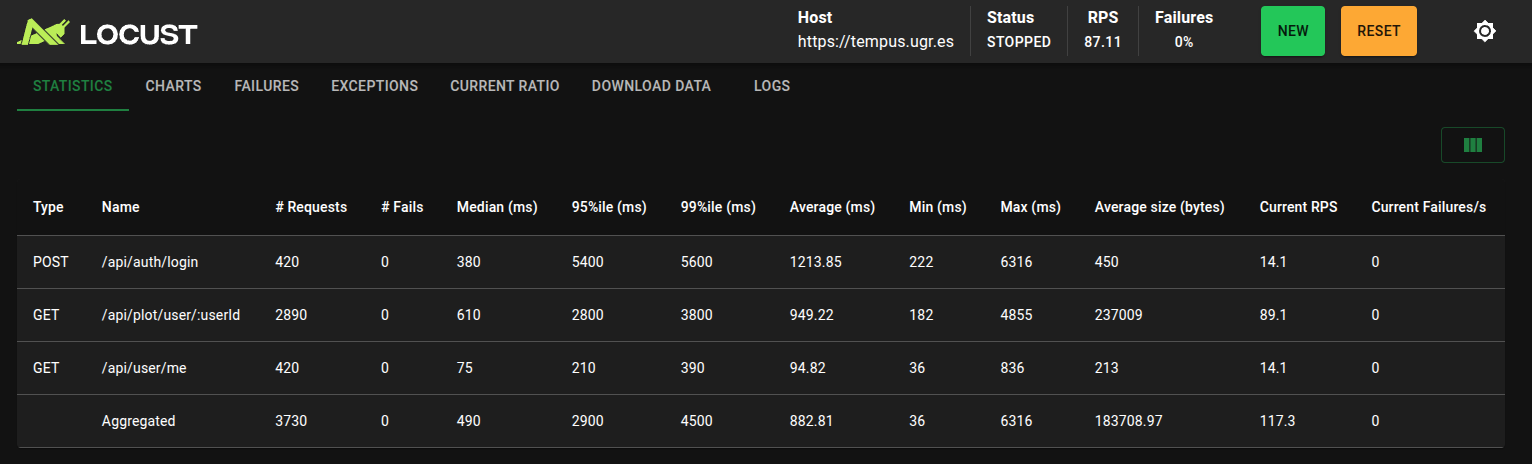
\includegraphics[width=0.9\textwidth]{figures/statis_1000_10_plots_tempus.png}
    \caption{Estadísticas para 1000 usuarios en la obtención de parcelas}
    \label{fig:statis_1000_10_plots_tempus}
\end{figure}

En este caso, se están realizando peticiones a 3 endpoints diferentes, pudiendo observar como el endpoint que obtiene todas las parcelas del usuario tiene los tiempos de respuesta más altos, pero sin
embargo, la gran mayoría de peticiones al endpoint del login tardan más en ser atendidas (95\% en 5s), causado probablemente por una cola saturada de peticiones.


